\section{Overall description}
\subsection{Product perspective}
	\subsubsection{System interfaces}
		The system we are to develop will have some external interfaces (represented in Figure \ref{fig:systemInterfaces}) to accomplish the goals stated in section 1.3.1\todo{reference?}.
		\begin{figure}[h]
			\centering
			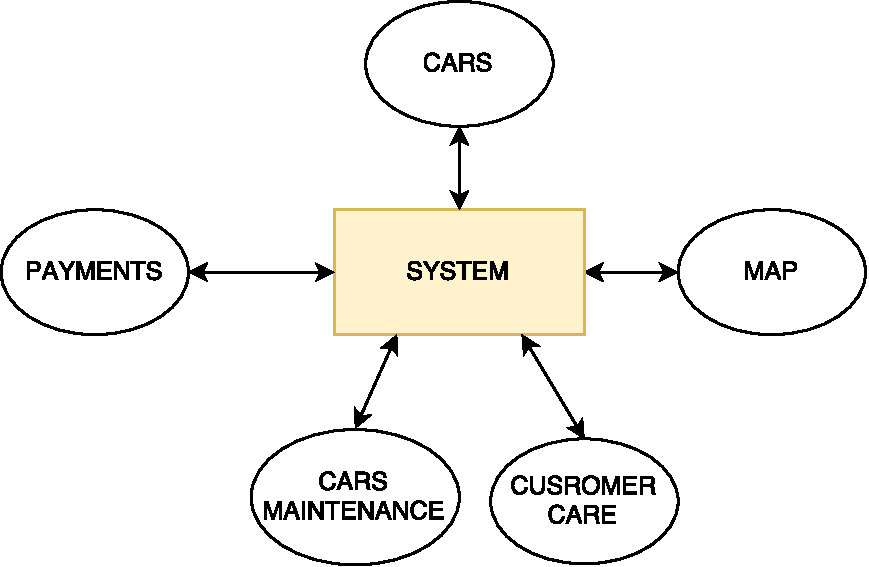
\includegraphics[scale=0.5]{system_blocks}
			\caption{
				\label{fig:systemInterfaces} 
				Overview of system interfaces
			}
		\end{figure}
	\paragraph{Payments}
	When a payment is required (e.g. when a user ends his rent) a request with all the details needed to complete the payment (i.d. name and surname of the user, due amount, credit card number etc.) is sent to an external payments system. Once the external system has completed the payment, it gives to our system a feedback of the payment process status so that we can take appropriate action.
	
	\paragraph{Customer care} Every time it is required a customer care service operator can contact a user. Customer care service operators can request and view all user details, their rent and payments history. Such operators can also ban or unban users from using the system, mark cars as not available and, in general, provide assistance to users during the rent.

	\paragraph{Maintenance} Every time maintenance for a car is required an external pool of maintenance operators is notified with GPS position of the car and a brief description of the problem.

	\paragraph{Map} GPS positions from cars and safe areas are displayed to all users, customer care operators and maintenance operators on a constantly updated map using an external reliable Geographic Information System.
	
	

\subsection{Domain assumption}
	We assume that these assumptions hold true in the domain of our system 
	\begin{itemize}
		\item GPS position is supposed to be accurate w.r.t. the defined areas
		\item GPS position and status of all cars is always available
		\item The user who reserves the car, will always be the person who drives it
		\item Users are legally allowed to drive cars (i.d. users have a proper driving license)
		\item Charging stations are always working and continuously monitored by the system
		\item Every time a user enters a car he ignites the engine
		\item All the data provided by users is correct and reliable
		\item 
	\end{itemize}